%% This document gives an example on how to use the ntnumasterthesis
%% LaTeX document class.

%% Use short name MACS, MIS, CIMET, MTDMT, MIXD or MIS  
%% Language english or norsk
%% a4paper or b5paper with oneside or twoside
\documentclass[MIXD,norsk,a4paper,oneside]{ntnuthesis/ntnuthesis}

\usepackage[T1]{fontenc}
\usepackage[utf8]{inputenc}     % For utf8 encoded .tex files allows norwegian characters in the files. This can be dangerous if you change to a differnt editor.
\usepackage[pdftex]{graphicx, hyperref}   % For cross references in pdf
\usepackage{color}              % For colouring text 
\hypersetup{colorlinks=true,     
		linkcolor=blue,          % color of internal links (change box color with linkbordercolor)
    citecolor=blue,        % color of links to bibliography
    filecolor=blue,      % color of file links
    urlcolor=blue           % color of external links
		}
\usepackage{csvsimple}  % for simple table reading and display
\usepackage{url}

% Set to true ONLY if using Harvard citation style
\newboolean{HarvardCitations}
\setboolean{HarvardCitations}{true} % false for computer science, true for interaction design and harvard style


\ifthenelse{\boolean{HarvardCitations}}{%
	\usepackage{natbib} % for Harvard names as citations.
}{%
	\usepackage[numbers]{natbib} % for Vancover numbers in bibliography
}



\begin{document}

\setthesistitle{Question analysis of coding questions on StackOverflow}
\setthesisauthor{130533 - Knut Lucas Andersen}
\setthesissupervisor{Assoc. Prof. Simon McCallum}
%\setthesissupervisorA{Prof. Jon Yngve Hardeberg}  % if you have a second supervisor add it like this

\setthesisHostInstitution{\NTNU}
%\setthesisHostInstitution{University of Eastern Finland}
%\setthesisHostInstitution{Universit\'e Jean Monnet Saint-Etienne}

%\setthesisjuryA{} %jury names
%\setthesisjuryB{} %jury names
%\setthesisjuryC{} %jury names
%\setthesisjuryD{} %jury names

\nmtkeywords{Question-answering, Artificial Intelligence, scikit-learn, Question-analysis, Programming}
%\nmtdesc{This is the short description of a masters thesis}


\setthesisdate{31-05-2016}
\setthesisyear{2016}
%\setthesiscampus{Gj\o{}vik}
 % this is the file which contains all the details about your thesis
\makefrontpages % make the frontpages
%this is the intro to the thesis
%\thesistitlepage % make the ordinary titlepage
\hypersetup{pageanchor=false}
%\include{summary}

% \addcontentsline{toc}{chapter}{Preface}
\chapter*{Preface}
This is my Master thesis concluding the two years spent at NTNU Gjøvik: Master Applied Computer Science - Web, Mobile, Games track. 
The thesis was carried out during the spring semester 2016, from January to the end of May. 

The main concept for the thesis was based on discussions with supervisor. The original plan was to create a Chat Agent that could answers students questions and give feedback 
to their question quality, by using Stack Overflow as a knowledge base. However, during the Master thesis project presentation, other professors noted that the scope of the 
project was to large for a Master thesis. The thesis were therefore narrowed down to focus on coding questions posted on Stack Overflow, in an attempt to evaluate question quality 
and predict whether or not it was a good programming question. 

%\begin{center}
%\thesiscampus, 
\thesisdate \\[1pc]
\\[1pc]
%\thesisauthor
%\end{center}

% \addcontentsline{toc}{chapter}{Acknowledgment}
\chapter*{Acknowledgment}
I would like to thank the following persons for their help and support during these years. It would not have been possible without them.

My supervisor, Simon McCallum, for understanding my difficult situation and for his patience and helpful advices on how to proceed so that I could complete my Master thesis.

Mariusz Nowostawski for his advice on how to get started with text processing and ideas for building the SVM model. 

Rune Hjelsvold for helpful advice in relation to text analysis.

My best friend, Njål Dolonen, for always being there for me, and helped me get through this.

My grandmother, Mimmi H. Underland, may she rest in peace. None of this would have been possible without your support, understanding, love and care. This is for you.

I would also thank my family and friends for believing in me and supporting me through this.

\begin{flushright}
K.L.A
\end{flushright}
% reset glossary
\glsresetall
% \addcontentsline{toc}{chapter}{Abstract}
\chapter*{Abstract}
\gls{so} is today for many developers a well known \gls{qa} system. 
However, \gls{so} has a high requirement to the questions and answers posted, which is reflected through their voting and reputation system. 
This peer-review processes can be used as an indicator to a questions quality, where questions with high up-votes can be defined as good questions.
In this thesis, a system has been developed using  \gls{ml} and \gls{svm} to see if it is possible to predict whether or not a new question will be 
considered as a good or bad question. 
\vspace{0.5em}\newline
This was achieved by using the \gls{se} data set, specifically using the one for \gls{so}. 
Questions were dived into two classes, where bad questions was question with a vote score below zero, and good questions were those above zero. 
Based on content in the various questions, a set of feature detectors was developed and tested against the raw data set. 
Surprisingly, the features actually lowered the accuracy score.
The raw, unprocessed classifier achieved a score of 79.90\%.
The classifier using Porter stemming and all features achieved a score of 75.97\%, and the classifier without stemming using all the features got a score of 79.12\%.


\begin{comment}

- Peer-review process \\
- Duplicates \\
- Bias \\
- Code examples (or lack thereof) \\
- Easier to spot bad questions \\
- Homework is not accepted \\



%This is a summary of the thesis including the conclusion of what was discovered.

% write messy notes now, cleanup afterwards; ignore if its too much in this round..

When you have a question you need an answer to, the solution many uses is to go online and use Google or another  type of search engine. 
However, the degree of difficulty in regards to finding an answer varies with the problem you need an answer to. 
Today, the Internet offers a wide range of resources to acquire new knowledge, everything from encyclopaedias to blogs, forums and Question-Answer communities. 
However, when you are writing code, or developing complex programs, it can be easy to get stuck and not figure out why something stopped working. 
\vspace{0.5em}\newline
Depending on the complexity of the problem, the only solution might be to go to an online community for help. 
One such community is StackExchange (consisting of 154 different communities), which is home to StackOverflow. 
A requirement for all StackExchange sites is that questions should be of good quality. The quality of a question is measured by use of votes and reputation. 
The votes are used to grade the question (or answer), whereas the reputation belongs to the user. 
\vspace{0.5em}\newline
% Re-write paragraph below later on
By using \gls{ml}, I wanted to see if it was possible to predict whether a new question would be viewed as a goodquestion on StackOverflow. 
This was done by using the dataset containing all posts on StackOverflow and the \gls{ml} method \gls{svm} (by using scikit-learn for Python). 
A lot of time was used understanding how scikit-learn worked and how to properly implement \gls{svm} to analyse the questions. 
\vspace{0.5em}\newline
One of the interesting finds was that the average down-vote score for 10,000 was -7. 
To develop the feature detectors, a total of 100 good and bad questions were looked at to see if there was anything that stood out. 
It was a lot harder to find anything significant for what was a good question, but it was easier to spot the bad questions 
(e.g. homework, no code-samples, no explanation to what had been done before, etc.).
\vspace{0.5em}\newline
% double check numbers later on to see that these are indeed correct Before any processing was done, the \gls{svm} had a vocabulary of 69,766 features. 
To reduce this amount, stop-words were added (reducing to 69,462 features) and removal of numbers and hexa-decimal values (27,624). 
The most significant change was when the document term frequency were set to 1\%, which gave a total of 440 features.

Write something more about feature detectors, results, etc. \\
Note! Not actual abstract, more of a general introduction to later narrow down to abstract

\end{comment}

\hypersetup{pageanchor=false}
% reset glossary
\glsresetall

\tableofcontents

\hypersetup{pageanchor=true}

% Comment with a percent to remove figures or tables:
\listoffigures
\listoftables


\include{introduction} % includes latex files from the same directory
\chapter{Packages}
\label{chap:packages}

The \texttt{ntnuthesis} is built upon the standard \LaTeX\
\texttt{report} class. All commands from the \texttt{report} class can
be used, with the two exceptions of \verb+\subsubsection+ and
\verb+\paragraph+. This is because there should only be three
levels of headings according to the guidelines~\cite{NTNUMaster}. 
It has been placed in a folder called \texttt{ntnuthesis} so that it does not
clutter your work.  You should not change anything in \texttt{ntnuthesis}

\section{Packages Used by ntnuthesis}
\label{sec:packages}

In addition to the \texttt{report} document class,
\texttt{ntnuthesis} makes direct use of the following packages
that must hence be present:
\begin{description}
	\item[geometry:] used for setting the sizes of the margins and
  	headers.
	\item[fontenc:] used with option \texttt{T1} for forcing the Cork font
  	encoding (necessary for the Charter font).
	\item[charter:] load Charter as the default font.
	\item[euler:] load the Euler math fonts.
	\item[bable:] for language handling.
\end{description}

\section{Other Relevant Packages}
\label{sec:otherpackages}

The author of a thesis might want to use a bunch of different packages
to those described in Section~\ref{sec:packages} in order to have all features needed for their document. 
In particular, it is advised to use the following:
\begin{description}
	\item[inputenc:] to allow \LaTeX\ to use more than 7-bit ASCII for its
	  input. Most often, the option \texttt{latin1} will do.
	\item[babel:] to load language specific strings. Reasonable options
	  include \texttt{british}, \texttt{american}, \texttt{norsk} and
	  \texttt{nynorsk}.
	\item[graphicx:] to include graphics.
	\item[hyperref:] this is a very nice package that makes cross links in
	  pdf documents. Use with option \texttt{dvips} or \texttt{pdftex}
	  in accordance with the driver that you use. Unfortunately, hyperref
	  is not completely bugfree\dots
\end{description}

We have web pages as well~\cite{HiG:Website}, and now games like Halo~\cite{Halo}. % could be called Methodology or methods or anyfile name 
\chapter{Structural Elements}
\label{chap:structural}

The title of the thesis should be set using the \verb+\thesistitle+
command, and the date of the thesis should be set using the
\verb+\thesisdate+ command. This makes the title and date appear in
the running header, like in this document.

\section{Page Layout}

The geometry of the page has been set using the \verb+\geometry+
command.

\section{Fonts}

Due to limited \LaTeX\ support for the Georgia font, Charter has been
chosen instead. For mathematical formula, the Euler fonts are used,
since they blend more nicely with the Charter than the standard
\LaTeX\ fonts: 
$$
 f(x) = \int_0^x g(\tau)\,d\tau
$$

For inline math you can use $\backslash{}($ and $\backslash{})$ for example \( f(x)= \frac{x^2}{1+x^2} \).  
This also allows you to use $\slash$ and $\backslash$. You need to include the \{\} when you want the special
character to have other letters immediately after it.

\section{Sectioning Commands}

The standard \LaTeX\ sectioning commands are used for both numbered
and unnumbered sections. The top level is given by the \verb+\chapter+
command. This starts a new right page. The two lower levels are
obtained using the \verb+\section+ and \verb+\subsection+ commands.
The standard \LaTeX\ \verb+\subsubsection+ and \verb+\paragraph+
commands have been disabled since their use is not encouraged by the
thesis guidelines. When you use these they will not be given numbers.  
They still appear in the document with highlighting but not in the 
table of contents.

\subsection{The subsection}

This is an example of a subsection.

\subsubsection{The subsubsection}

This is an example of a subsubsection.

\paragraph{The paragraph}

This is an example of a paragraph with a heading.

\section{Floats (Figures and Tables)}
\label{sec:floats}

Figures are placed in the \texttt{figure} environment. An example is
shown in Figure~\ref{fig:example}. %notice the ~ in between figure and the \ref. it stops latex from splitting the number and word over a line.
Tables are placed in the \texttt{table} environment. An example is given in
Table~\ref{tab:example}. Figures and tables float freely around in the
document in accordance with standard \LaTeX\ behavior.

\begin{figure}[tbp]  %t top, b bottom, p page | you can also use h to try to get the figure to appear at the current location
  \centering
  \includegraphics[width=.5\textwidth]{figures/example_fig}
  \caption[An example figure.]{An example figure. If the caption is
    shorter than one line, it is centered. If it goes over more than
    one line, it is left and right justified. Furthermore, it is
    suggested that an alternative short caption is given in order to
    produce a good list of figures.}
  \label{fig:example}
\end{figure}

\begin{table}[tbp]
  \centering
  \begin{tabular}{c|c}
    Age  & IQ  \\ 
    \hline
    10   & 100 \\
    20   & 100 \\
    30   & 150 \\
    40   & 100 \\
    50   & 100
  \end{tabular}
  \caption{An example table.}
  \label{tab:example}
\end{table}

The captions are placed \emph{below} both for the figures and the
tables. The caption is set in 9pt. If the caption is shorter than one
line, it is centered.

\section{Quotes}
\label{sec:Quotes} % this allows you to refer to this section number using \ref{sec:Quotes}

Quotes are inserted using the standard \LaTeX\ \texttt{quote}
environment. The environment has been changed so that a 9pt font is
used:

\begin{quote}
  ``And I looked, and, behold, a whirlwind came out of the north, a
  great cloud, and a fire infolding itself, and a brightness was about
  it, and out of the midst thereof as the colour of amber, out of the
  midst of the fire. Also out of the midst thereof came the likeness
  of four living creatures.''
\end{quote}

\section{Lists}
\label{sec:lists}

Point lists and enumerated lists are made by using the standard
\texttt{itemize} and \texttt{enumerate} environments, respectively.
The spacing is going to be changed in accordance with the specification. For
\texttt{itemize}, the results look like this:
\begin{itemize}
	\item First item.
	\item Second item. Here I will put some long text, just to illustrate.
	  Here I will put some long text, just to illustrate. Here I will put
	  some long text, just to illustrate. Here I will put some long text,
	  just to illustrate.
	\item Third item also has subitems:
	  \begin{itemize}
		  \item First subitem.
		  \item Second subitem.
		  \item Third subitem.
	  \end{itemize}
\end{itemize}
and for \texttt{enumerate} like this:
\begin{enumerate}
	\item First item.
	\item Second item. Here I will put some long text, just to illustrate.
	  Here I will put some long text, just to illustrate. Here I will put
	  some long text, just to illustrate. Here I will put some long text,
	  just to illustrate.
	\item Third item also has subitems:
	  \begin{enumerate}
		  \item First subitem.
		  \item Second subitem.
		  \item Third subitem.
	  \end{enumerate}
\end{enumerate}

You may also want to use descriptive lists
\begin{description}
	\item[First] the first item.
	\item[Second] the second item. Here I will put some long text, just to illustrate.
	  Here I will put some long text, just to illustrate. Here I will put
	  some long text, just to illustrate. Here I will put some long text,
	  just to illustrate.
	\item [What now] the third item also has subitems:
	  \begin{enumerate}
		  \item First subitem.
		  \item Second subitem.
		  \item Third subitem.
	  \end{enumerate}
\end{description}


\section{Bibliographic References}

You should cite articles~\cite{Askvall1985}, books~\cite{Card1983},
anthologies~\cite{Lancaster1985} and web publications~\cite{Meldon1997}
like this. There is always an issue referencing web pages. Currently
we suggest that you use the HiG Website~\cite{HiG:Website}.


A particular bibliography style file for NTNU named
\texttt{ntnuthesis.bst} has been developed based upon the
standard Bib\TeX\ \texttt{unsrt} style.
 % could be results


\ifthenelse{\boolean{HarvardCitations}}{%
	\bibliographystyle{agsm} % used for Harvard style references. Names - Humanities & Interaction Design
}{%
	\bibliographystyle{ntnuthesis/ntnuthesis} %used for Vancover style references. Numbers - Computer Science & Physics
}

\bibliography{MastersExample}

\appendix
%%%%%%%%%%%%%%%%%%%%%%%%%%%%%%%%%%%%%%%%%%%%%%%%%%%%%%%%%%%%%
%% APPENDICES
%%%%%%%%%%%%%%%%%%%%%%%%%%%%%%%%%%%%%%%%%%%%%%%%%%%%%%%%%%%%%
\appendix

\chapter{Appendix}
\label{app:acronyms}
%% acronyms
\printindex
\printglossaries

%\section{Data sets/Statistical Overview}
%\label{app:data_sets}

\clearpage
\section{MySQL Database}
\label{app:mysql_database}
% image of the mysql database
\begin{figure}[ht]
	\centering
    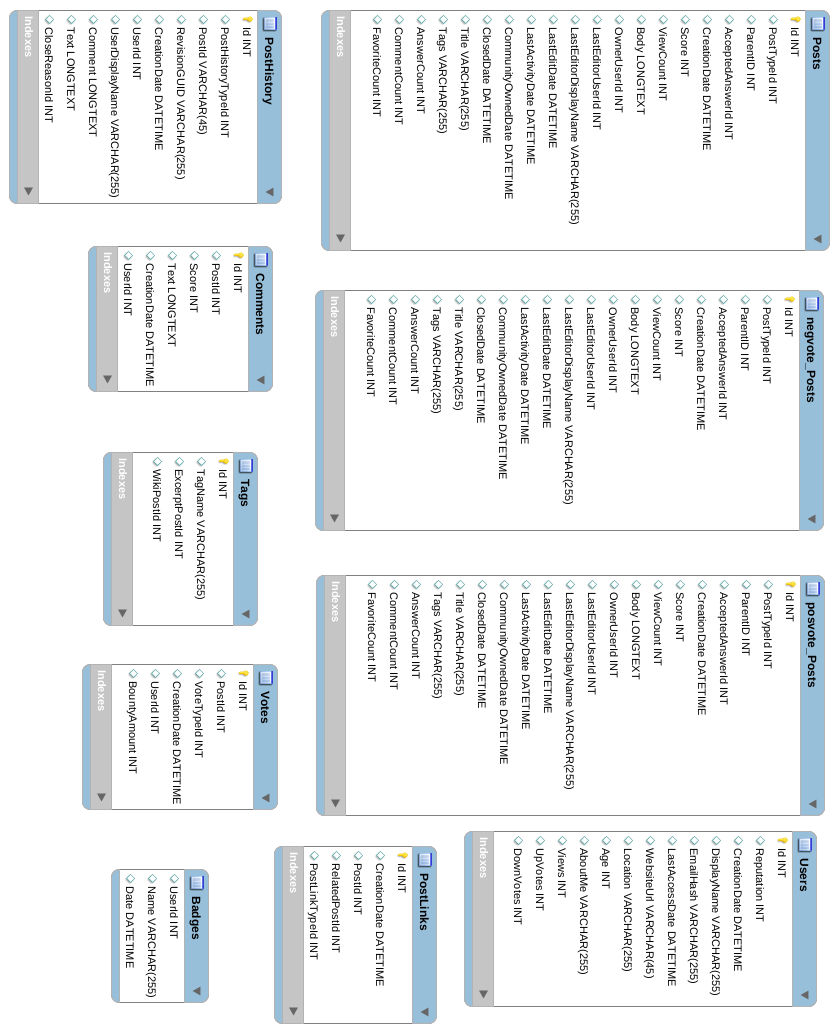
\includegraphics[width=0.8\textwidth]{so_database}
	\caption{MySQL Database used for dataset}
	\label{fig:mysql_database}
\end{figure}

\clearpage
\section{Tex.Stack Exchange: Data set and Features}
\label{app:tables_tex}

%description
\begin{table}[!h]%[tbp]
	\centering
	\begin{tabular}{| c | c | c | c | c | c |}
		\hline
		~				& Amount		& Oldest		& Newest		& Vote (lowest)		& Vote (highest)	\\ \hline
		Votes < 0		& 93			& 22.08.2010	& 10.09.2014	& -14				& -1				\\ \hline
		Votes = 0		& 5,078			& 26.07.2010	& 14.09.2014	& 0					& 0					\\ \hline
		Votes > 0		& 65,919		& 18.08.2008	& 14.09.2014	& 1					& 448				\\ \hline
		All questions	& 71,090 		& 18.08.2008	& 14.09.2014	& -14				& 448				\\ \hline
	\end{tabular}
\caption{Overview of the questions in the Tex.StackExhange (August 2015 data set)}
\label{tab:dataset_overview_tex}
\end{table}

% editor space
\begin{table}[!h]%[tbp]
	\centering
	\begin{tabular}{| c | c | c |}
		\hline
		~ 			& Unprocessed		& Features	\\ \hline
		Score 		& 0.99				& 0.99		\\ \hline
		C			& 1					& 1			\\ \hline
		Kernel		& Linear			& Linear	\\ \hline
	\end{tabular}
\caption{Comparison of raw data set (unprocessed) and feature detectors for Tex.StackExhange (August 2015 data set). Vote score was < 0 for bad and > +7 for good.}
\label{tab:singular_feature_detector_tex}
\end{table}

% description
\begin{table}[!h]%[tbp]
	\centering
	\begin{tabular}{| c | c | c |}
		\hline
		Actual 		& Predicted: -1	& Predicted: 1	\\ \hline
		-1			& 0			& 15				\\ \hline
		1			& 0			& 2004				\\ \hline
	\end{tabular}
	\caption{Confusion Matrix for Tex.StackExhange.}
	\label{tab:confusion_matrix_tex}
\end{table}

% description
\begin{table}[!h]%[tbp]
	\centering
	\begin{tabular}{| c | c | c | c | c |}
		\hline
		~				& Precision		& Recall	& F1-score		& Support	\\ \hline
		-1      		& 0.00			& 0.00		& 0.00			& 15		\\ \hline
		1       		& 0.99			& 1.00		& 1.00			& 2004		\\ \hline
		avg / total		& 0.99			& 0.99		& 0.99			& 2019		\\ \hline
	\end{tabular}
	\caption{Classification report for Tex.StackExhange (August 2015 data set).}
	\label{tab:tex_classification_report}
\end{table}

\clearpage
\section{Confusion Matrices for Stack Overflow}
\label{app:confusion_matrix}
\subsection{Confusion matrices for unprocessed and all feature detectors}

\begin{table}[!htb]
	\caption{Confusion Matrix for unprocessed data set and all feature detectors using the same parameters.}
	\begin{minipage}{.5\linewidth}
		\caption{Unprocessed dataset}
		\centering
		\begin{tabular}{| c | c | c |}
			\hline
			Actual 		& Predicted: -1	& Predicted: 1	\\ \hline
			-1			& 1591			& 403			\\ \hline
			1			& 401			& 1605			\\ \hline
		\end{tabular}
	\end{minipage}%
	\begin{minipage}{.5\linewidth}
		\centering
		\caption{All features}
		\begin{tabular}{| c | c | c |}
			\hline
			Actual 		& Predicted: -1	& Predicted: 1	\\ \hline
			-1			& 1558			& 436			\\ \hline
			1			& 401			& 1605			\\ \hline
		\end{tabular}
	\end{minipage} 
	\begin{minipage}{.5\linewidth}
		\caption{Code blocks}
		\centering
		\begin{tabular}{| c | c | c |}
			\hline
			Actual 		& Predicted: -1	& Predicted: 1	\\ \hline
			-1			& 1547			& 420			\\ \hline
			1			& 413			& 1593			\\ \hline
		\end{tabular}
	\end{minipage}%
	\begin{minipage}{.5\linewidth}
		\centering
		\caption{Hexadecimal}
		\begin{tabular}{| c | c | c |}
			\hline
			Actual 		& Predicted: -1	& Predicted: 1	\\ \hline
			-1			& 1591			& 403			\\ \hline
			1			& 401			& 1605			\\ \hline
		\end{tabular}
	\end{minipage} 
	\begin{minipage}{.5\linewidth}
		\caption{Homework}
		\centering
		\begin{tabular}{| c | c | c |}
			\hline
			Actual 		& Predicted: -1	& Predicted: 1	\\ \hline
			-1			& 1590			& 404			\\ \hline
			1			& 400			& 1606			\\ \hline
		\end{tabular}
	\end{minipage}%
	\begin{minipage}{.5\linewidth}
		\centering
		\caption{Links}
		\begin{tabular}{| c | c | c |}
			\hline
			Actual 		& Predicted: -1	& Predicted: 1	\\ \hline
			-1			& 1548			& 410			\\ \hline
			1			& 416			& 1590			\\ \hline
		\end{tabular}
	\end{minipage} 	
	\begin{minipage}{.5\linewidth}
		\centering
		\caption{Numerical}
		\begin{tabular}{| c | c | c |}
			\hline
			Actual 		& Predicted: -1	& Predicted: 1	\\ \hline
			-1			& 1591			& 403			\\ \hline
			1			& 375			& 1631			\\ \hline
		\end{tabular}
	\end{minipage}%	
	\begin{minipage}{.5\linewidth}
		\caption{Tags}
		\centering
		\begin{tabular}{| c | c | c |}
			\hline
			Actual 		& Predicted: -1	& Predicted: 1	\\ \hline
			-1			& 1508			& 486			\\ \hline
			1			& 467			& 1539			\\ \hline
		\end{tabular}
	\end{minipage}
\end{table}	


\begin{table}[!htb]
	\caption{Confusion Matrix for all features, with and without stemming.}
	\begin{minipage}{.5\linewidth}
		\caption{With stemming}
		\centering
		\begin{tabular}{| c | c | c |}
			\hline
			Actual 		& Predicted: -1	& Predicted: 1	\\ \hline
			-1			& 1558			& 436				\\ \hline
			1			& 525			& 1481				\\ \hline
		\end{tabular}
	\end{minipage}%
	\begin{minipage}{.5\linewidth}
		\centering
		\caption{Without stemming}
		\begin{tabular}{| c | c | c |}
			\hline
			Actual 		& Predicted: -1	& Predicted: 1	\\ \hline
			-1			& 1567			& 427				\\ \hline
			1			& 408			& 1598				\\ \hline
		\end{tabular}
	\end{minipage} 
\end{table}	
\begin{table}[!htb]
	\caption{Confusion Matrix for the SGD classifier, with loss='log'.}
	\begin{minipage}{.5\linewidth}
		\caption{Unprocessed}
		\centering
		\begin{tabular}{| c | c | c |}
			\hline
			Actual 		& Predicted: -1	& Predicted: 1	\\ \hline
			-1			& 1610			& 384			\\ \hline
			1			& 594			& 1412			\\ \hline
		\end{tabular}
	\end{minipage}%
	\begin{minipage}{.5\linewidth}
		\caption{All features with stemming}
		\centering
		\begin{tabular}{| c | c | c |}
			\hline
			Actual 		& Predicted: -1	& Predicted: 1	\\ \hline
			-1			& 1607			& 387			\\ \hline
			1			& 418			& 1588			\\ \hline
		\end{tabular}
	\end{minipage} 
\end{table}	

\begin{comment}
\clearpage
%\subsection{Confusion matrix for singular feature detectors - all questions}

\begin{table}[!htb]
	\caption{Confusion Matrix for singular feature detectors, based on all questions in the data set.}	
	\begin{minipage}{.5\linewidth}
		\caption{Code blocks}
		\centering
		\begin{tabular}{| c | c | c |}
			\hline
			Actual 		& Predicted: -1	& Predicted: 1	\\ \hline
			-1			& 1547			& 420			\\ \hline
			1			& 413			& 1593			\\ \hline
		\end{tabular}
	\end{minipage}%
	\begin{minipage}{.5\linewidth}
		\centering
		\caption{Hexadecimal}
		\begin{tabular}{| c | c | c |}
			\hline
			Actual 		& Predicted: -1	& Predicted: 1	\\ \hline
			-1			& 1591			& 403			\\ \hline
			1			& 401			& 1605			\\ \hline
		\end{tabular}
	\end{minipage} 
	\begin{minipage}{.5\linewidth}
		\caption{Homework}
		\centering
		\begin{tabular}{| c | c | c |}
			\hline
			Actual 		& Predicted: -1	& Predicted: 1	\\ \hline
			-1			& 1590			& 404			\\ \hline
			1			& 400			& 1606			\\ \hline
		\end{tabular}
	\end{minipage}%
	\begin{minipage}{.5\linewidth}
		\centering
		\caption{Links}
		\begin{tabular}{| c | c | c |}
			\hline
			Actual 		& Predicted: -1	& Predicted: 1	\\ \hline
			-1			& 1548			& 410			\\ \hline
			1			& 416			& 1590			\\ \hline
		\end{tabular}
	\end{minipage} 	
	\begin{minipage}{.5\linewidth}
		\centering
		\caption{Numerical}
		\begin{tabular}{| c | c | c |}
			\hline
			Actual 		& Predicted: -1	& Predicted: 1	\\ \hline
			-1			& 1591			& 403			\\ \hline
			1			& 375			& 1631			\\ \hline
		\end{tabular}
	\end{minipage}%	
	\begin{minipage}{.5\linewidth}
		\caption{Tags}
		\centering
		\begin{tabular}{| c | c | c |}
			\hline
			Actual 		& Predicted: -1	& Predicted: 1	\\ \hline
			-1			& 1508			& 486			\\ \hline
			1			& 467			& 1539			\\ \hline
		\end{tabular}
	\end{minipage}
\end{table}	

\end{comment}

\clearpage
\subsection{Confusion matrices for singular feature detectors - occurrence only}
\label{app:conf_matrix_singular_only}

\begin{table}[!htb]
	\caption{Confusion Matrix for singular feature detectors, only for questions containing it.}
	\begin{minipage}{.5\linewidth}
		\caption{Unprocessed}
		\centering
		\begin{tabular}{| c | c | c |}
			\hline
			Actual 		& Predicted: -1	& Predicted: 1	\\ \hline
			-1			& 786			& 202			\\ \hline
			1			& 215			& 768				\\ \hline
		\end{tabular}
	\end{minipage}%
	\begin{minipage}{.5\linewidth}
		\centering
		\caption{Code blocks}
		\begin{tabular}{| c | c | c |}
			\hline
			Actual 		& Predicted: -1	& Predicted: 1	\\ \hline
			-1			& 793			& 195			\\ \hline
			1			& 218			& 765				\\ \hline
		\end{tabular}
	\end{minipage}
	\begin{minipage}{.5\linewidth}
		\caption{Unprocessed}
		\centering
		\begin{tabular}{| c | c | c |}
			\hline
			Actual 		& Predicted: -1	& Predicted: 1	\\ \hline
			-1			& 21			& 0			\\ \hline
			1			& 6				& 5				\\ \hline
		\end{tabular}
	\end{minipage}%
	\begin{minipage}{.5\linewidth}
		\centering
		\caption{Hexadecimal}
		\begin{tabular}{| c | c | c |}
			\hline
			Actual 		& Predicted: -1	& Predicted: 1	\\ \hline
			-1			& 21			& 0				\\ \hline
			1			& 6				& 5				\\ \hline
		\end{tabular}
	\end{minipage} 	
	\begin{minipage}{.5\linewidth}
		\centering
		\caption{Unprocessed}
		\begin{tabular}{| c | c | c |}
			\hline
			Actual 		& Predicted: -1	& Predicted: 1	\\ \hline
			-1			& 52			& 4			\\ \hline
			1			& 8				& 11		\\ \hline
		\end{tabular}
	\end{minipage} 	%
	\begin{minipage}{.5\linewidth}
		\caption{Homework}
		\centering
		\begin{tabular}{| c | c | c |}
			\hline
			Actual 		& Predicted: -1	& Predicted: 1	\\ \hline
			-1			& 50			& 6 			\\ \hline
			1			& 7 			& 12			\\ \hline
		\end{tabular}
	\end{minipage}
	\begin{minipage}{.5\linewidth}
		\caption{Unprocessed}
		\centering
		\begin{tabular}{| c | c | c |}
			\hline
			Actual 		& Predicted: -1	& Predicted: 1	\\ \hline
			-1			& 95			& 56			\\ \hline
			1			& 28			& 337			\\ \hline
		\end{tabular}
	\end{minipage}%
	\begin{minipage}{.5\linewidth}
		\centering
		\caption{Links}
		\begin{tabular}{| c | c | c |}
			\hline
			Actual 		& Predicted: -1	& Predicted: 1	\\ \hline
			-1			& 87			& 64			\\ \hline
			1			& 30			& 335			\\ \hline
		\end{tabular}
	\end{minipage} 
	\begin{minipage}{.5\linewidth}
		\caption{Unprocessed}
		\centering
		\begin{tabular}{| c | c | c |}
			\hline
			Actual 		& Predicted: -1	& Predicted: 1	\\ \hline
			-1			& 1044			& 110			\\ \hline
			1			& 247			& 404			\\ \hline
		\end{tabular}
	\end{minipage}%
	\begin{minipage}{.5\linewidth}
		\centering
		\caption{Numerical}
		\begin{tabular}{| c | c | c |}
			\hline
			Actual 		& Predicted: -1	& Predicted: 1	\\ \hline
			-1			& 1043			& 111			\\ \hline
			1			& 256			& 395			\\ \hline
		\end{tabular}
	\end{minipage} 	
	\begin{minipage}{.5\linewidth}
		\centering
		\caption{Unprocessed}
		\begin{tabular}{| c | c | c |}
			\hline
			Actual 		& Predicted: -1	& Predicted: 1	\\ \hline
			-1			& 1559			& 426			\\ \hline
			1			& 398			& 1611			\\ \hline
		\end{tabular}
	\end{minipage}%
	\begin{minipage}{.5\linewidth}
		\caption{Tags}
		\centering
		\begin{tabular}{| c | c | c |}
			\hline
			Actual 		& Predicted: -1	& Predicted: 1	\\ \hline
			-1			& 1487			& 498			\\ \hline
			1			& 442			& 1567			\\ \hline
		\end{tabular}
	\end{minipage}
	\begin{minipage}{.5\linewidth}
		\caption{Unprocessed}
		\centering
		\begin{tabular}{| c | c | c |}
			\hline
			Actual 		& Predicted: -1	& Predicted: 1	\\ \hline
			-1			& 1284			& 387			\\ \hline
			1			& 342			& 1499			\\ \hline
		\end{tabular}
	\end{minipage}%
	\begin{minipage}{.5\linewidth}
		\caption{All features}
		\centering
		\begin{tabular}{| c | c | c |}
			\hline
			Actual 		& Predicted: -1	& Predicted: 1	\\ \hline
			-1			& 1268			& 403			\\ \hline
			1			& 329			& 1512			\\ \hline
		\end{tabular}
	\end{minipage}
\end{table}	

\begin{comment}
\section{Classification report for Stack Overflow}

\begin{table}[!htb]
	\caption{Classification report for unprocessed data set and all feature detectors using the same parameters.}
	\begin{minipage}{.5\linewidth}
		\caption{Unprocessed dataset}
		\centering
		\begin{tabular}{| c | c | c | c | c |}
			\hline
			~				& Precision		& Recall	& F1-score		& Support	\\ \hline
			-1      		& xxxx			& xxxx		& xxxx			& xxxx		\\ \hline
			1       		& xxxx			& xxxx		& 1x00			& xxxx		\\ \hline
			avg/total		& xxxx			& xxxx		& xxxx			& xxxx		\\ \hline
		\end{tabular}
	\end{minipage}%
	\begin{minipage}{.5\linewidth}
		\centering
		\caption{All features}
		\begin{tabular}{| c | c | c | c | c |}
			\hline
			Precision		& Recall	& F1-score		& Support	\\ \hline
			xxxx			& xxxx		& xxxx			& xxxx		\\ \hline
			xxxx			& xxxx		& 1x00			& xxxx		\\ \hline
			xxxx			& xxxx		& xxxx			& xxxx		\\ \hline
		\end{tabular}
	\end{minipage} 
	\begin{minipage}{.5\linewidth}
		\caption{Code blocks}
		\centering
		\begin{tabular}{| c | c | c | c | c |}
			\hline
			~				& Precision		& Recall	& F1-score		& Support	\\ \hline
			-1      		& xxxx			& xxxx		& xxxx			& xxxx		\\ \hline
			1       		& xxxx			& xxxx		& 1x00			& xxxx		\\ \hline
			avg / total		& xxxx			& xxxx		& xxxx			& xxxx		\\ \hline
		\end{tabular}
	\end{minipage}%
	\begin{minipage}{.5\linewidth}
		\centering
		\caption{Hexadecimal}
		\begin{tabular}{| c | c | c | c | c |}
			\hline
			~				& Precision		& Recall	& F1-score		& Support	\\ \hline
			-1      		& xxxx			& xxxx		& xxxx			& xxxx		\\ \hline
			1       		& xxxx			& xxxx		& 1x00			& xxxx		\\ \hline
			avg / total		& xxxx			& xxxx		& xxxx			& xxxx		\\ \hline
		\end{tabular}
	\end{minipage} 
	\begin{minipage}{.5\linewidth}
		\caption{Homework}
		\centering
		\begin{tabular}{| c | c | c | c | c |}
			\hline
			~				& Precision		& Recall	& F1-score		& Support	\\ \hline
			-1      		& xxxx			& xxxx		& xxxx			& xxxx		\\ \hline
			1       		& xxxx			& xxxx		& 1x00			& xxxx		\\ \hline
			avg / total		& xxxx			& xxxx		& xxxx			& xxxx		\\ \hline
		\end{tabular}
	\end{minipage}%
	\begin{minipage}{.5\linewidth}
		\centering
		\caption{Links}
		\begin{tabular}{| c | c | c | c | c |}
			\hline
			~				& Precision		& Recall	& F1-score		& Support	\\ \hline
			-1      		& xxxx			& xxxx		& xxxx			& xxxx		\\ \hline
			1       		& xxxx			& xxxx		& 1x00			& xxxx		\\ \hline
			avg / total		& xxxx			& xxxx		& xxxx			& xxxx		\\ \hline
		\end{tabular}
	\end{minipage} 	
	\begin{minipage}{.5\linewidth}
		\centering
		\caption{Numerical}
		\begin{tabular}{| c | c | c | c | c |}
			\hline
			~				& Precision		& Recall	& F1-score		& Support	\\ \hline
			-1      		& xxxx			& xxxx		& xxxx			& xxxx		\\ \hline
			1       		& xxxx			& xxxx		& 1x00			& xxxx		\\ \hline
			avg / total		& xxxx			& xxxx		& xxxx			& xxxx		\\ \hline
		\end{tabular}
	\end{minipage}%	
	\begin{minipage}{.5\linewidth}
		\caption{Tags}
		\centering
		\begin{tabular}{| c | c | c | c | c |}
			\hline
			~				& Precision		& Recall	& F1-score		& Support	\\ \hline
			-1      		& xxxx			& xxxx		& xxxx			& xxxx		\\ \hline
			1       		& xxxx			& xxxx		& 1x00			& xxxx		\\ \hline
			avg / total		& xxxx			& xxxx		& xxxx			& xxxx		\\ \hline
		\end{tabular}
	\end{minipage}
\end{table}	


\begin{table}[!htb]
	\caption{Classification report for all features, with and without stemming.}
	\begin{minipage}{.5\linewidth}
		\caption{With stemming}
		\centering
		\begin{tabular}{| c | c | c | c | c |}
			\hline
			~				& Precision		& Recall	& F1-score		& Support	\\ \hline
			-1      		& xxxx			& xxxx		& xxxx			& xxxx		\\ \hline
			1       		& xxxx			& xxxx		& 1x00			& xxxx		\\ \hline
			avg / total		& xxxx			& xxxx		& xxxx			& xxxx		\\ \hline
		\end{tabular}
	\end{minipage}%
	\begin{minipage}{.5\linewidth}
		\centering
		\caption{Without stemming}
		\begin{tabular}{| c | c | c | c | c |}
			\hline
			~				& Precision		& Recall	& F1-score		& Support	\\ \hline
			-1      		& xxxx			& xxxx		& xxxx			& xxxx		\\ \hline
			1       		& xxxx			& xxxx		& 1x00			& xxxx		\\ \hline
			avg / total		& xxxx			& xxxx		& xxxx			& xxxx		\\ \hline
		\end{tabular}
	\end{minipage} 
\end{table}	
\begin{table}[!htb]
	\caption{Confusion Matrix for the SGD classifier, with loss='log'.}
	\begin{minipage}{.5\linewidth}
		\caption{Unprocessed}
		\centering
		\begin{tabular}{| c | c | c | c | c |}
			\hline
			~				& Precision		& Recall	& F1-score		& Support	\\ \hline
			-1      		& xxxx			& xxxx		& xxxx			& xxxx		\\ \hline
			1       		& xxxx			& xxxx		& 1x00			& xxxx		\\ \hline
			avg / total		& xxxx			& xxxx		& xxxx			& xxxx		\\ \hline
		\end{tabular}
	\end{minipage}%
	\begin{minipage}{.5\linewidth}
		\caption{All features with stemming}
		\centering
		\begin{tabular}{| c | c | c | c | c |}
			\hline
			~				& Precision		& Recall	& F1-score		& Support	\\ \hline
			-1      		& xxxx			& xxxx		& xxxx			& xxxx		\\ \hline
			1       		& xxxx			& xxxx		& 1x00			& xxxx		\\ \hline
			avg / total		& xxxx			& xxxx		& xxxx			& xxxx		\\ \hline
		\end{tabular}
	\end{minipage} 
\end{table}	

\clearpage
\subsection{Classification report for singular feature detectors - occurrence only}

\begin{table}[!htb]
	\caption{Classification report for singular feature detectors, only for questions containing it.}
	\begin{minipage}{.5\linewidth}
		\caption{Unprocessed}
		\centering
		\begin{tabular}{| c | c | c | c | c |}
			\hline
			~				& Precision		& Recall	& F1-score		& Support	\\ \hline
			-1      		& xxxx			& xxxx		& xxxx			& xxxx		\\ \hline
			1       		& xxxx			& xxxx		& 1x00			& xxxx		\\ \hline
			avg / total		& xxxx			& xxxx		& xxxx			& xxxx		\\ \hline
		\end{tabular}
	\end{minipage}%
	\begin{minipage}{.5\linewidth}
		\centering
		\caption{Code blocks}
		\begin{tabular}{| c | c | c | c | c |}
			\hline
			~				& Precision		& Recall	& F1-score		& Support	\\ \hline
			-1      		& xxxx			& xxxx		& xxxx			& xxxx		\\ \hline
			1       		& xxxx			& xxxx		& 1x00			& xxxx		\\ \hline
			avg / total		& xxxx			& xxxx		& xxxx			& xxxx		\\ \hline
		\end{tabular}
	\end{minipage}
	\begin{minipage}{.5\linewidth}
		\caption{Unprocessed}
		\centering
		\begin{tabular}{| c | c | c | c | c |}
			\hline
			~				& Precision		& Recall	& F1-score		& Support	\\ \hline
			-1      		& xxxx			& xxxx		& xxxx			& xxxx		\\ \hline
			1       		& xxxx			& xxxx		& 1x00			& xxxx		\\ \hline
			avg / total		& xxxx			& xxxx		& xxxx			& xxxx		\\ \hline
		\end{tabular}
	\end{minipage}%
	\begin{minipage}{.5\linewidth}
		\centering
		\caption{Hexadecimal}
		\begin{tabular}{| c | c | c | c | c |}
			\hline
			~				& Precision		& Recall	& F1-score		& Support	\\ \hline
			-1      		& xxxx			& xxxx		& xxxx			& xxxx		\\ \hline
			1       		& xxxx			& xxxx		& 1x00			& xxxx		\\ \hline
			avg / total		& xxxx			& xxxx		& xxxx			& xxxx		\\ \hline
		\end{tabular}
	\end{minipage} 	
	\begin{minipage}{.5\linewidth}
		\centering
		\caption{Unprocessed}
		\begin{tabular}{| c | c | c | c | c |}
			\hline
			~				& Precision		& Recall	& F1-score		& Support	\\ \hline
			-1      		& xxxx			& xxxx		& xxxx			& xxxx		\\ \hline
			1       		& xxxx			& xxxx		& 1x00			& xxxx		\\ \hline
			avg / total		& xxxx			& xxxx		& xxxx			& xxxx		\\ \hline
		\end{tabular}
	\end{minipage}%
	\begin{minipage}{.5\linewidth}
		\caption{Homework}
		\centering
		\begin{tabular}{| c | c | c | c | c |}
			\hline
			~				& Precision		& Recall	& F1-score		& Support	\\ \hline
			-1      		& xxxx			& xxxx		& xxxx			& xxxx		\\ \hline
			1       		& xxxx			& xxxx		& 1x00			& xxxx		\\ \hline
			avg / total		& xxxx			& xxxx		& xxxx			& xxxx		\\ \hline
		\end{tabular}
	\end{minipage}
	\begin{minipage}{.5\linewidth}
		\caption{Unprocessed}
		\centering
		\begin{tabular}{| c | c | c | c | c |}
			\hline
			~				& Precision		& Recall	& F1-score		& Support	\\ \hline
			-1      		& xxxx			& xxxx		& xxxx			& xxxx		\\ \hline
			1       		& xxxx			& xxxx		& 1x00			& xxxx		\\ \hline
			avg / total		& xxxx			& xxxx		& xxxx			& xxxx		\\ \hline
		\end{tabular}
	\end{minipage}%
	\begin{minipage}{.5\linewidth}
		\centering
		\caption{Links}
		\begin{tabular}{| c | c | c | c | c |}
			\hline
			~				& Precision		& Recall	& F1-score		& Support	\\ \hline
			-1      		& xxxx			& xxxx		& xxxx			& xxxx		\\ \hline
			1       		& xxxx			& xxxx		& 1x00			& xxxx		\\ \hline
			avg / total		& xxxx			& xxxx		& xxxx			& xxxx		\\ \hline
		\end{tabular}
	\end{minipage} 
	\begin{minipage}{.5\linewidth}
		\caption{Unprocessed}
		\centering
		\begin{tabular}{| c | c | c | c | c |}
			\hline
			~				& Precision		& Recall	& F1-score		& Support	\\ \hline
			-1      		& xxxx			& xxxx		& xxxx			& xxxx		\\ \hline
			1       		& xxxx			& xxxx		& 1x00			& xxxx		\\ \hline
			avg / total		& xxxx			& xxxx		& xxxx			& xxxx		\\ \hline
		\end{tabular}
	\end{minipage}%
	\begin{minipage}{.5\linewidth}
		\centering
		\caption{Numerical}
		\begin{tabular}{| c | c | c | c | c |}
			\hline
			~				& Precision		& Recall	& F1-score		& Support	\\ \hline
			-1      		& xxxx			& xxxx		& xxxx			& xxxx		\\ \hline
			1       		& xxxx			& xxxx		& 1x00			& xxxx		\\ \hline
			avg / total		& xxxx			& xxxx		& xxxx			& xxxx		\\ \hline
		\end{tabular}
	\end{minipage} 	
	\begin{minipage}{.5\linewidth}
		\centering
		\caption{Unprocessed}
		\begin{tabular}{| c | c | c | c | c |}
			\hline
			~				& Precision		& Recall	& F1-score		& Support	\\ \hline
			-1      		& xxxx			& xxxx		& xxxx			& xxxx		\\ \hline
			1       		& xxxx			& xxxx		& 1x00			& xxxx		\\ \hline
			avg / total		& xxxx			& xxxx		& xxxx			& xxxx		\\ \hline
		\end{tabular}
	\end{minipage}%
	\begin{minipage}{.5\linewidth}
		\caption{Tags}
		\centering
		\begin{tabular}{| c | c | c | c | c |}
			\hline
			~				& Precision		& Recall	& F1-score		& Support	\\ \hline
			-1      		& xxxx			& xxxx		& xxxx			& xxxx		\\ \hline
			1       		& xxxx			& xxxx		& 1x00			& xxxx		\\ \hline
			avg / total		& xxxx			& xxxx		& xxxx			& xxxx		\\ \hline
		\end{tabular}
	\end{minipage}
	\begin{minipage}{.5\linewidth}
		\caption{Unprocessed}
		\centering
		\begin{tabular}{| c | c | c | c | c |}
			\hline
			~				& Precision		& Recall	& F1-score		& Support	\\ \hline
			-1      		& xxxx			& xxxx		& xxxx			& xxxx		\\ \hline
			1       		& xxxx			& xxxx		& 1x00			& xxxx		\\ \hline
			avg / total		& xxxx			& xxxx		& xxxx			& xxxx		\\ \hline
		\end{tabular}
	\end{minipage}%
	\begin{minipage}{.5\linewidth}
		\caption{All features}
		\centering
		\begin{tabular}{| c | c | c | c | c |}
			\hline
			~				& Precision		& Recall	& F1-score		& Support	\\ \hline
			-1      		& xxxx			& xxxx		& xxxx			& xxxx		\\ \hline
			1       		& xxxx			& xxxx		& 1x00			& xxxx		\\ \hline
			avg / total		& xxxx			& xxxx		& xxxx			& xxxx		\\ \hline
		\end{tabular}
	\end{minipage}
\end{table}	


\begin{lstlisting}[keepspaces=True]
Classification Report:
			Precision	Recall		F1-score	Support
-1.0			0.79		0.76		0.78		1671
1.0			0.79		0.82		0.81		1841
avg / total		0.79		0.79      	0.79		3512



td-10000-Unprocessed
--------------------
Classification Report:
			Precision	Recall		F1-score	Support
-1       0.80      0.80      0.80      1994
1       0.80      0.80      0.80      2006
avg / total       0.80      0.80      0.80      4000


Creating singular feature detector:  Code blocks
-----------------------------------------------
Classification Report:
			Precision	Recall		F1-score	Support
-1       0.79      0.79      0.79      1994
1       0.79      0.79      0.79      2006
avg / total       0.79      0.79      0.79      4000


Creating singular feature detector:  Links
-------------------------------------------
Classification Report:
			Precision	Recall		F1-score	Support
-1       0.79      0.79      0.79      1994
1       0.80      0.79      0.79      2006
avg / total       0.79      0.79      0.79      4000


Creating singular feature detector:  Homework
----------------------------------------
Classification Report:
			Precision	Recall		F1-score	Support
-1       0.80      0.80      0.80      1994
1       0.80      0.80      0.80      2006
avg / total       0.80      0.80      0.80      4000


Creating singular feature detector:  Numerical
----------------------------------------
Classification Report:
			Precision	Recall		F1-score	Support
-1       0.81      0.80      0.80      1994
1       0.80      0.81      0.81      2006
avg / total       0.81      0.81      0.81      4000


Creating singular feature detector:  Hexadecimal
----------------------------------------
Classification Report:
			Precision	Recall		F1-score	Support
-1       0.80      0.80      0.80      1994
1       0.80      0.80      0.80      2006
avg / total       0.80      0.80      0.80      4000


Creating singular feature detector:  Tags
----------------------------------------
Classification Report:
			Precision	Recall		F1-score	Support
-1       0.76      0.76      0.76      1994
1       0.76      0.77      0.76      2006
avg / total       0.76      0.76      0.76      4000


All features using 10k-unprocessed settings
----------------------------------------
Classification Report:
			Precision	Recall		F1-score	Support
-1       0.80      0.78      0.79      1994
1       0.79      0.80      0.79      2006
avg / total       0.79      0.79      0.79      4000


Creating model without stemming, using exhaustive search
------------------------------------------------------------
Classification Report:
			Precision	Recall		F1-score	Support
-1       0.79      0.79      0.79      1994
1       0.79      0.80      0.79      2006
avg / total       0.79      0.79      0.79      4000


td-10k
----------------------------------------
Classification Report:
			Precision	Recall		F1-score	Support
-1       0.75      0.78      0.76      1994
1       0.77      0.74      0.76      2006
avg / total       0.76      0.76      0.76      4000


td-10k-no-stemming
---------------------------------------------
Classification Report:
			Precision	Recall		F1-score	Support
-1       0.79      0.79      0.79      1994
1       0.79      0.80      0.79      2006
avg / total       0.79      0.79      0.79      4000


10k-sgd-loss-log
----------------------------------------
Classification Report:
			Precision	Recall		F1-score	Support
-1       0.73      0.81      0.77      1994
1       0.79      0.70      0.74      2006
avg / total       0.76      0.76      0.75      4000


10k-unprocessed-sgd
------------------
Classification Report:
			Precision	Recall		F1-score	Support
-1       0.79      0.81      0.80      1994
1       0.80      0.79      0.80      2006
avg / total       0.80      0.80      0.80      4000


10k-unprocessed-sgd-log-loss
------------------
Classification Report:
			Precision	Recall		F1-score	Support
-1       0.79      0.81      0.80      1994
1       0.80      0.79      0.80      2006
avg / total       0.80      0.80      0.80      4000


td-10k-all-features-occurrence-only
------------------
Classification Report:
			Precision	Recall		F1-score	Support
-1.0       0.79      0.76      0.78      1671
1.0       0.79      0.82      0.81      1841
avg / total       0.79      0.79      0.79      3512


td-10l-unprocessed-codeblocks
------------------------------------
Classification Report:
			Precision	Recall		F1-score	Support
-1.0       0.78      0.80      0.79       988
1.0       0.80      0.78      0.79       983
avg / total       0.79      0.79      0.79      1971


td-10l-unprocessed-hexadecimal
------------------------------------
Classification Report:
			Precision	Recall		F1-score	Support
-1.0       0.78      1.00      0.88        21
1.0       1.00      0.45      0.62        11
avg / total       0.85      0.81      0.79        32


td-10l-unprocessed-homework
------------------------------------
Classification Report:
			Precision	Recall		F1-score	Support
-1.0       0.88      0.89      0.88        56
1.0       0.67      0.63      0.65        19
avg / total       0.82      0.83      0.83        75


td-10l-unprocessed-links
------------------------------------
Classification Report:
			Precision	Recall		F1-score	Support
-1.0       0.74      0.58      0.65       151
1.0       0.84      0.92      0.88       365
avg / total       0.81      0.82      0.81       516


td-10l-unprocessed-numeric
------------------------------------
Classification Report:
			Precision	Recall		F1-score	Support
-1.0       0.80      0.90      0.85      1154
1.0       0.78      0.61      0.68       651
avg / total       0.79      0.80      0.79      1805


td-10l-unprocessed-tags
------------------------------------
Classification Report:
			Precision	Recall		F1-score	Support
-1.0       0.77      0.75      0.76      1985
1.0       0.76      0.78      0.77      2009
avg / total       0.76      0.76      0.76      3994
td-10l-unprocessed-all-features
------------------------------------
Classification Report:
			Precision	Recall		F1-score	Support
-1.0       0.79      0.77      0.78      1671
1.0       0.79      0.81      0.80      1841
avg / total       0.79      0.79      0.79      3512


td-10l-unprocessed-up-codeblocks
------------------------------------
Classification Report:
			Precision	Recall		F1-score	Support
-1.0       0.79      0.80      0.79       988
1.0       0.79      0.78      0.79       983
avg / total       0.79      0.79      0.79      1971


td-10l-unprocessed-up-hex
------------------------------------
Classification Report:
			Precision	Recall		F1-score	Support
-1.0       0.78      1.00      0.88        21
1.0       1.00      0.45      0.62        11
avg / total       0.85      0.81      0.79        32


td-10l-unprocessed-up-homework
------------------------------------
Classification Report:
precision    	recall  	f1-score   	support
-1.0       			0.87      		0.93      	0.90        56
1.0       			0.73      		0.58      	0.65        19
avg / total       	0.83     	 	0.84      	0.83        75


td-10l-unprocessed-up-links
------------------------------------
Classification Report:
			Precision	Recall		F1-score	Support
-1.0       0.77      0.63      0.69       151
1.0       0.86      0.92      0.89       365
avg / total       0.83      0.84      0.83       516


td-10l-unprocessed-up-numeric
------------------------------------
Classification Report:
			Precision	Recall		F1-score	Support
-1.0       0.81      0.90      0.85      1154
1.0       0.79      0.62      0.69       651
avg / total       0.80      0.80      0.80      1805


td-10l-unprocessed-up-tags
------------------------------------
Classification Report:
			Precision	Recall		F1-score	Support
-1.0       0.80      0.79      0.79      1985
1.0       0.79      0.80      0.80      2009
avg / total       0.79      0.79      0.79      3994
\end{lstlisting}

\end{comment}
				
\clearpage
\section{Various screenshots}
\label{app:various_screenshots}
% image of how it looked when using all tags
\begin{figure}[ht]
	\centering
	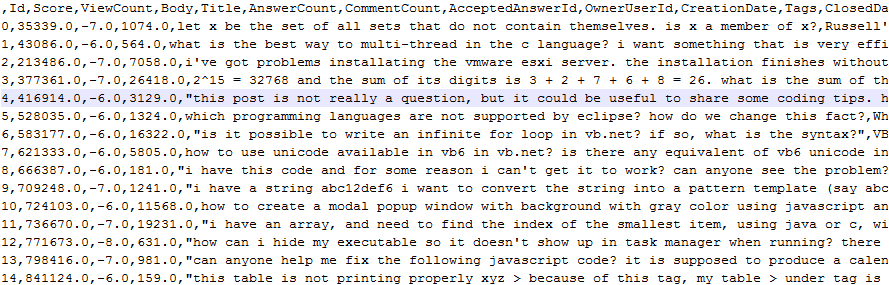
\includegraphics[width=0.8\textwidth]{tag_features_raw}
	\caption{Question without external tags detected.}
	\label{fig:tag_features_raw}
\end{figure}
\begin{figure}[ht]
	\centering
	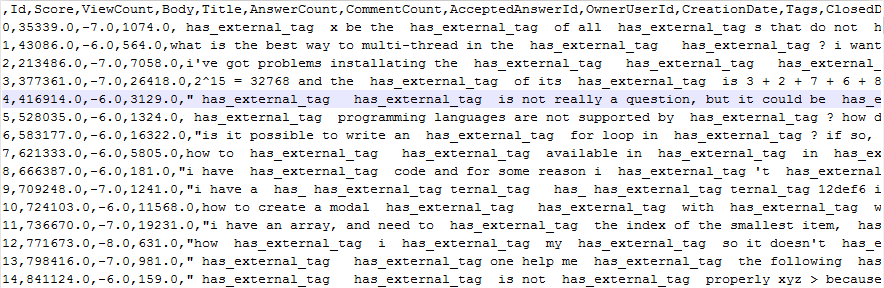
\includegraphics[width=0.8\textwidth]{tag_features_external}
	\caption{Question with external tags detected.}
	\label{fig:tag_features_external}
\end{figure}

\clearpage
\section{Scikit-learns roadmap - Choosing the right estimator}
\label{app:ml_map}
% image of the cheat-sheet from scikit-learn
\begin{figure}[ht]
	\centering
	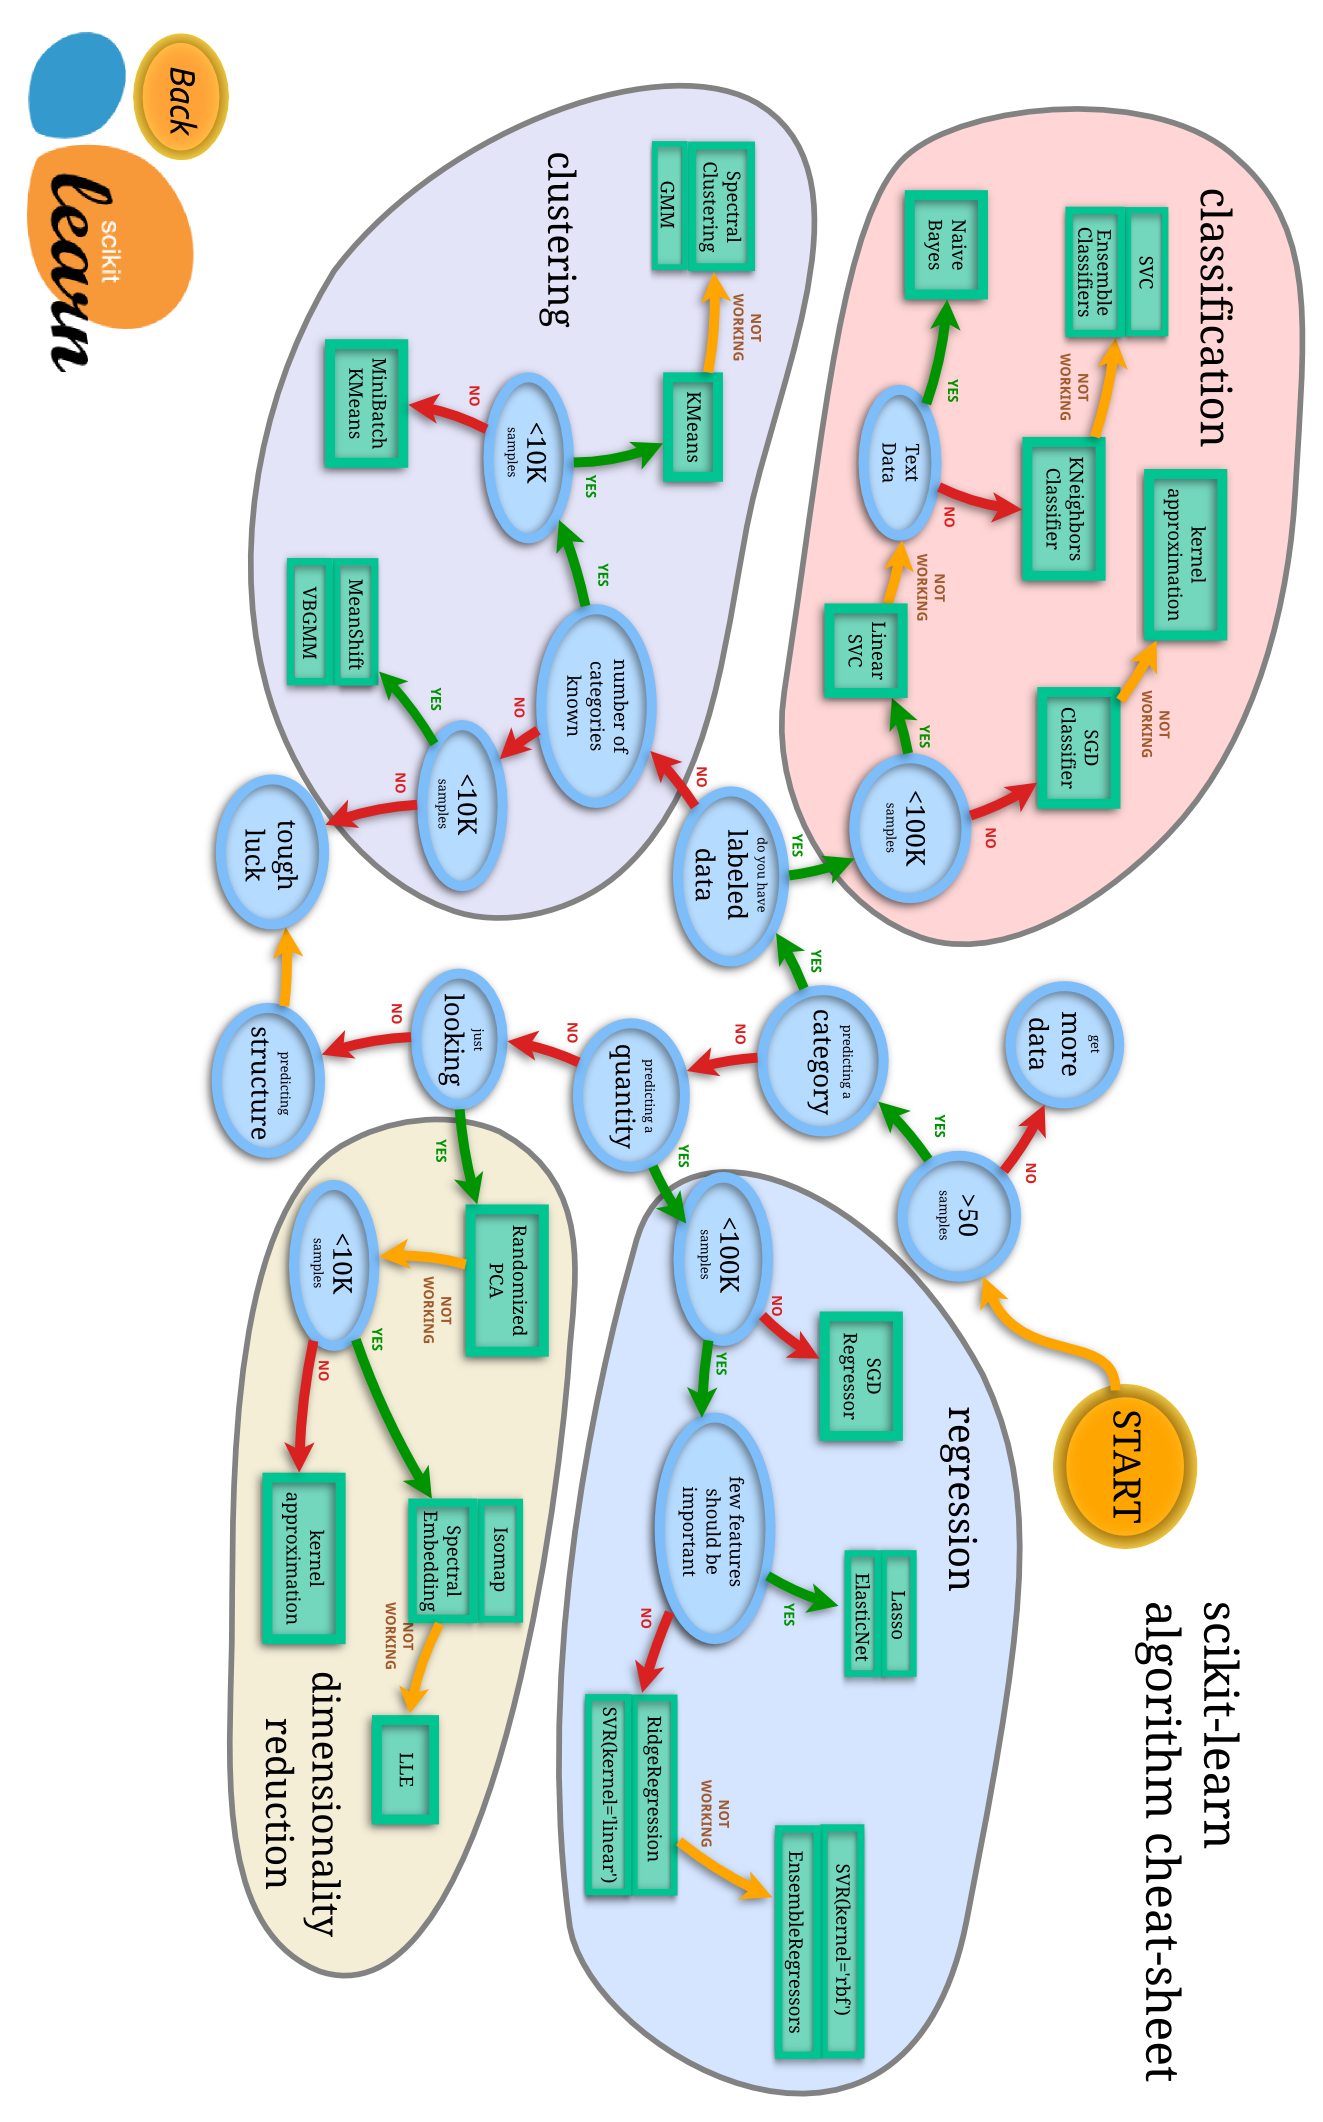
\includegraphics[width=0.645\textwidth]{ml_map}
	\caption[Choosing the right estimator]{Choosing the right estimator \cite{Scikitlearn.org2016i}.}
	\label{fig:ml_map}
\end{figure}

\clearpage
\section{Quick installation guide for Windows x64}
\label{app:installation_windows}
Since Python is much more adapted to *nix systems then Windows, I decided to write a short guide on how to install Python 3.5 and Scikit-learn on Windows. 
This guide is provided as-is, and I make no guarantees that this will result in a functioning installation, but it should at least reduce the problems. 
A presumption here is that the operative system is Windows x64 (if you have x86, you can ignore all the x64 settings).
Before installing anything, download the following:
\begin{itemize}
	\item Python: \url{https://www.python.org/downloads/windows/}. \\
	Select the Python version with "Windows x86-64" in its name.
	\item CygWin: \url{https://cygwin.com/}
	\item MinGW: \url{http://www.mingw.org/}
	\item MySQL connector for Python (Git; only needed for running this project): \\
	\url{https://github.com/mysql/mysql-connector-python}.
	\item x64 version of Numpy and Scipy \cite{Codementor.io2015,Gehrcke2015}: \\ 
	\url{http://www.lfd.uci.edu/~gohlke/pythonlibs/}. \\ 
	The latest available versions at the time of writing is "\emph{numpy-1.11.1rc1+mkl-cp35-cp35m-win\_amd64.whl}" and "\emph{scipy-0.17.1-cp35-cp35m-win\_amd64.whl}".
	\item Scikit-learn (Git): \url{https://github.com/scikit-learn/scikit-learn}
	\item If you do not have a version of Microsoft Visual Studio installed, you need to install Visual Studio 2013 or newer (because compiler requires it)\footnote{
		"vcvarsall.bat needed for python to compile missing from visual studio 2015": \\
		\url{http://stackoverflow.com/q/33323172}
	}.
\end{itemize}
% editor space
\begin{enumerate}
	\item Install Python, update pip, and install these packages: \\
	\emph{pip install -U bs4 pandas nltk matplotlib cython nose nosetests}
	\item Install MinGW.
	 Thereafter select "mingw32-base" under "MinGW Base System".
	In addition, under "MinGW Base System", select all belonging to Class "bin" and "dll"
	\item Install CygWin. 
	During installation, you will be asked what you want to install. 
	Select all entries that contains "gcc", "mingw64", "make", "automake", "lapack" and "openblas".
	The GCC-compilers are used in combination with MinGW, because Scikit-learn needs Fortran, Lapack and OpenBlas for \emph{make} to succeed.
	\item Change to folder with the x64 version of Numpy and Scipy, and install them~\cite{Codementor.io2015,Gehrcke2015}: \\
	\emph{pip install "numpy-1.11.1rc1+mkl-cp35-cp35m-win\_amd64.whl"} \\
	Verify installation: 1. \emph{python}, 2. \emph{import numpy}, 3. \emph{numpy.\_\_version\_\_}. \\
	\emph{pip install "scipy-0.17.1-cp35-cp35m-win\_amd64.whl"} and verify using the same steps, swapping numpy with scipy.
	\item Start CygWin (run as administrator), change to directory containing Scikit-learn and run the following commands: \\
	\emph{python setup.py build}  and \emph{python setup.py install}.
	\item If you want to use \gls{nltk}, you need to run \emph{python}, \emph{import nltk} and \emph{ntlk.download()} to download the corpus.
\end{enumerate}


% backup of various created tables


\begin{comment}

td-10000-Unprocessed
--------------------
Confusion matrix for test set classification:
[[1591  403]
[ 401 1605]]
Accuracy score for test set:
0.799
Classification Report:
			Precision	Recall		F1-score	Support

-1       0.80      0.80      0.80      1994
1       0.80      0.80      0.80      2006

avg / total       0.80      0.80      0.80      4000


Creating singular feature detector:  Code blocks
-----------------------------------------------
Confusion matrix for test set classification:
[[1574  420]
[ 413 1593]]
Accuracy score for test set:
0.79175
Classification Report:
			Precision	Recall		F1-score	Support

-1       0.79      0.79      0.79      1994
1       0.79      0.79      0.79      2006

avg / total       0.79      0.79      0.79      4000


Creating singular feature detector:  Links
-------------------------------------------
Confusion matrix for test set classification:
[[1584  410]
[ 416 1590]]
Accuracy score for test set:
0.7935
Classification Report:
			Precision	Recall		F1-score	Support

-1       0.79      0.79      0.79      1994
1       0.80      0.79      0.79      2006

avg / total       0.79      0.79      0.79      4000


Creating singular feature detector:  Homework
----------------------------------------
Confusion matrix for test set classification:
[[1590  404]
[ 400 1606]]
Accuracy score for test set:
0.799
Classification Report:
			Precision	Recall		F1-score	Support

-1       0.80      0.80      0.80      1994
1       0.80      0.80      0.80      2006

avg / total       0.80      0.80      0.80      4000


Creating singular feature detector:  Numerical
----------------------------------------
Confusion matrix for test set classification:
[[1591  403]
[ 375 1631]]
Accuracy score for test set:
0.8055
Classification Report:
			Precision	Recall		F1-score	Support

-1       0.81      0.80      0.80      1994
1       0.80      0.81      0.81      2006

avg / total       0.81      0.81      0.81      4000


Creating singular feature detector:  Hexadecimal
----------------------------------------
Confusion matrix for test set classification:
[[1591  403]
[ 401 1605]]
Accuracy score for test set:
0.799
Classification Report:
			Precision	Recall		F1-score	Support

-1       0.80      0.80      0.80      1994
1       0.80      0.80      0.80      2006

avg / total       0.80      0.80      0.80      4000


Creating singular feature detector:  Tags
----------------------------------------
Confusion matrix for test set classification:
[[1508  486]
[ 467 1539]]
Accuracy score for test set:
0.76175
Classification Report:
			Precision	Recall		F1-score	Support

-1       0.76      0.76      0.76      1994
1       0.76      0.77      0.76      2006

avg / total       0.76      0.76      0.76      4000


All features using 10k-unprocessed settings
----------------------------------------
Confusion matrix for test set classification:
[[1558  436]
[ 401 1605]]
Accuracy score for test set:
0.79075
Classification Report:
			Precision	Recall		F1-score	Support

-1       0.80      0.78      0.79      1994
1       0.79      0.80      0.79      2006

avg / total       0.79      0.79      0.79      4000


Creating model without stemming, using exhaustive search
------------------------------------------------------------
Confusion matrix for test set classification:
[[1567  427]
[ 408 1598]]
Accuracy score for test set:
0.79125
Classification Report:
			Precision	Recall		F1-score	Support

-1       0.79      0.79      0.79      1994
1       0.79      0.80      0.79      2006

avg / total       0.79      0.79      0.79      4000


td-10k
----------------------------------------
Confusion matrix for test set classification:
[[1558  436]
[ 525 1481]]
Accuracy score for test set:
0.75975
Classification Report:
			Precision	Recall		F1-score	Support

-1       0.75      0.78      0.76      1994
1       0.77      0.74      0.76      2006

avg / total       0.76      0.76      0.76      4000


td-10k-no-stemming
---------------------------------------------
Confusion matrix for test set classification:
[[1568  426]
[ 408 1598]]
Accuracy score for test set:
0.7915
Classification Report:
			Precision	Recall		F1-score	Support

-1       0.79      0.79      0.79      1994
1       0.79      0.80      0.79      2006

avg / total       0.79      0.79      0.79      4000


10k-sgd-loss-log
----------------------------------------
Confusion matrix for test set classification:
[[1610  384]
[ 594 1412]]
Accuracy score for test set:
0.7555
Classification Report:
			Precision	Recall		F1-score	Support

-1       0.73      0.81      0.77      1994
1       0.79      0.70      0.74      2006

avg / total       0.76      0.76      0.75      4000


10k-unprocessed-sgd
------------------
Confusion matrix for test set classification:
[[1607  387]
[ 418 1588]]
Accuracy score for test set:
0.79875
Classification Report:
			Precision	Recall		F1-score	Support

-1       0.79      0.81      0.80      1994
1       0.80      0.79      0.80      2006

avg / total       0.80      0.80      0.80      4000


10k-unprocessed-sgd-log-loss
------------------
Confusion matrix for test set classification:
[[1607  387]
[ 418 1588]]
Accuracy score for test set:
0.79875
Classification Report:
			Precision	Recall		F1-score	Support

-1       0.79      0.81      0.80      1994
1       0.80      0.79      0.80      2006

avg / total       0.80      0.80      0.80      4000


td-10k-all-features-occurrence-only
------------------
Confusion matrix for test set classification:
[[1268  403]
[ 329 1512]]
Accuracy score for test set:
0.791571753986
Classification Report:
			Precision	Recall		F1-score	Support

-1.0       0.79      0.76      0.78      1671
1.0       0.79      0.82      0.81      1841

avg / total       0.79      0.79      0.79      3512


td-10l-unprocessed-codeblocks
------------------------------------
Confusion matrix for test set classification:
[[793 195]
[218 765]]
Accuracy score for test set:
0.790461694571
Classification Report:
			Precision	Recall		F1-score	Support

-1.0       0.78      0.80      0.79       988
1.0       0.80      0.78      0.79       983

avg / total       0.79      0.79      0.79      1971


td-10l-unprocessed-hexadecimal
------------------------------------
Confusion matrix for test set classification:
[[21  0]
[ 6  5]]
Accuracy score for test set:
0.8125
Classification Report:
			Precision	Recall		F1-score	Support

-1.0       0.78      1.00      0.88        21
1.0       1.00      0.45      0.62        11

avg / total       0.85      0.81      0.79        32


td-10l-unprocessed-homework
------------------------------------
Confusion matrix for test set classification:
[[50  6]
[ 7 12]]
Accuracy score for test set:
0.826666666667
Classification Report:
			Precision	Recall		F1-score	Support

-1.0       0.88      0.89      0.88        56
1.0       0.67      0.63      0.65        19

avg / total       0.82      0.83      0.83        75


td-10l-unprocessed-links
------------------------------------
Confusion matrix for test set classification:
[[ 87  64]
[ 30 335]]
Accuracy score for test set:
0.817829457364
Classification Report:
			Precision	Recall		F1-score	Support

-1.0       0.74      0.58      0.65       151
1.0       0.84      0.92      0.88       365

avg / total       0.81      0.82      0.81       516


td-10l-unprocessed-numeric
------------------------------------
Confusion matrix for test set classification:
[[1043  111]
[ 256  395]]
Accuracy score for test set:
0.796675900277
Classification Report:
			Precision	Recall		F1-score	Support

-1.0       0.80      0.90      0.85      1154
1.0       0.78      0.61      0.68       651

avg / total       0.79      0.80      0.79      1805


td-10l-unprocessed-tags
------------------------------------
Confusion matrix for test set classification:
[[1487  498]
[ 442 1567]]
Accuracy score for test set:
0.764646970456
Classification Report:
			Precision	Recall		F1-score	Support

-1.0       0.77      0.75      0.76      1985
1.0       0.76      0.78      0.77      2009

avg / total       0.76      0.76      0.76      3994

td-10l-unprocessed-all-features
------------------------------------
Confusion matrix for test set classification:
[[1284  387]
[ 342 1499]]
Accuracy score for test set:
0.792425968109
Classification Report:
			Precision	Recall		F1-score	Support

-1.0       0.79      0.77      0.78      1671
1.0       0.79      0.81      0.80      1841

avg / total       0.79      0.79      0.79      3512


td-10l-unprocessed-up-codeblocks
------------------------------------
Confusion matrix for test set classification:
[[786 202]
[215 768]]
Accuracy score for test set:
0.788432267884
Classification Report:
			Precision	Recall		F1-score	Support

-1.0       0.79      0.80      0.79       988
1.0       0.79      0.78      0.79       983

avg / total       0.79      0.79      0.79      1971


td-10l-unprocessed-up-hex
------------------------------------
Confusion matrix for test set classification:
[[21  0]
[ 6  5]]
Accuracy score for test set:
0.8125
Classification Report:
			Precision	Recall		F1-score	Support

-1.0       0.78      1.00      0.88        21
1.0       1.00      0.45      0.62        11

avg / total       0.85      0.81      0.79        32


td-10l-unprocessed-up-homework
------------------------------------
Confusion matrix for test set classification:
[[52  4]
[ 8 11]]
Accuracy score for test set:
0.84
Classification Report:
					precision    	recall  	f1-score   	support

-1.0       			0.87      		0.93      	0.90        56
1.0       			0.73      		0.58      	0.65        19

avg / total       	0.83     	 	0.84      	0.83        75


td-10l-unprocessed-up-links
------------------------------------
Confusion matrix for test set classification:
[[ 95  56]
[ 28 337]]
Accuracy score for test set:
0.837209302326
Classification Report:
			Precision	Recall		F1-score	Support

-1.0       0.77      0.63      0.69       151
1.0       0.86      0.92      0.89       365

avg / total       0.83      0.84      0.83       516


td-10l-unprocessed-up-numeric
------------------------------------
Confusion matrix for test set classification:
[[1044  110]
[ 247  404]]
Accuracy score for test set:
0.802216066482
Classification Report:
			Precision	Recall		F1-score	Support

-1.0       0.81      0.90      0.85      1154
1.0       0.79      0.62      0.69       651

avg / total       0.80      0.80      0.80      1805


td-10l-unprocessed-up-tags
------------------------------------
Confusion matrix for test set classification:
[[1559  426]
[ 398 1611]]
Accuracy score for test set:
0.793690535804
Classification Report:
			Precision	Recall		F1-score	Support

-1.0       0.80      0.79      0.79      1985
1.0       0.79      0.80      0.80      2009

avg / total       0.79      0.79      0.79      3994

\end{comment}


\begin{comment}
\begin{table}[!htb]
\caption{Confusion Matrix for xxxxx.}
\begin{minipage}{.5\linewidth}
\caption{Unprocessed dataset}
\centering
\begin{tabular}{| c | c | c |}
\hline
Actual 		& Predicted: -1	& Predicted: 1	\\ \hline
-1			& xx			& xx			\\ \hline
1			& xx			& xx			\\ \hline
\end{tabular}
\end{minipage}%
\begin{minipage}{.5\linewidth}
\centering
\caption{All features}
\begin{tabular}{| c | c | c |}
\hline
Actual 		& Predicted: -1	& Predicted: 1	\\ \hline
-1			& xx			& xx			\\ \hline
1			& xx			& xx			\\ \hline
\end{tabular}
\end{minipage} 
\end{table}	
\end{comment}
\begin{comment}
% potentially flip this, and this as a Score X feature (since all kernel values were the same)
% something like "Comparison ..., with Kernel = RBF, Gamma = gamma and C = c
% and the table having features as rows, and score X unprocessed as column
\begin{table}[tbp]
\centering
\begin{tabular}{| c | c | c | c | c | c | c | c |}
\hline
~ 					& Code block	& Numerical		& Hexadecimal	& Homework		& Link 		& Tags	\\ \hline
Score 				& 0.783			& 0.796			& 0.793			& 0.794			& 0.795 	& 0.757	\\ \hline
C					& 1000			& 1000			& 1000			& 1000			& 1000 		& 1000	\\ \hline
Gamma ($\gamma$)	& 0.001			& 0.001			& 0.001			& 0.001			& 0.001 	& 0.001	\\ \hline
Kernel				& RBF			& RBF			& RBF			& RBF			& RBF 		& RBF	\\ \hline
\end{tabular}
\caption{Comparison of raw data set (unprocessed) and singular feature detectors}
%\label{tab:singular_feature_detector_so2}
\end{table}

\begin{table}[tbp]
\centering
\begin{tabular}{| c | c | c | c | c |}
\hline
~				& Votes < 0			& Votes = 0			& Votes > 0		& All			\\ \hline
Amount			& 659,955			& 5,256,105			& 5,286,971		& 11,203,031	\\ \hline
Oldest			& 06.08.2008		& 06.08.2008		& 31.07.2008	& 31.07.2008 	\\ \hline
Newest			& 06.03.2016		& 06.03.2016		& 06.03.2016	& 06.03.2016	\\ \hline
Vote (lowest)	& -147				& 0					& 1				& -147	 		\\ \hline
Vote (highest)	& -1				& 0					& 13845			& 13845	 		\\ \hline
\end{tabular}
\caption{Overview of the Stack Overflow dataset.}
%\label{tab:dataset_overview_so2}
\end{table}

Amount of features before anything was done to the text: 69766 - CountVectorizer(analyzer='word') - \%
Amount of features after adding stop word (English): 69462 - CountVectorizer(analyzer='word', stop\_words="english") - \%
Amount of features after removing code block, hexadecimals and numeric values: 27624 - \%
Amount of features after setting minimum document frequency: 440 - CountVectorizer(analyzer='word', min\_df=0.01, stop_words='english') - \%


Originally tagged questions as good/bad, but then switched to +/-1 due to considering switching to LibSVM.
\end{comment}


\end{document}
